Neben der Studie der Niederländischen Bank gibt es ein veröffentlichtes Life Cycle Assessment, welches die Umweltauswirkungen des gesamten Euro-Bargeld-Systems mit dem Bitcoin-System vergleicht. Die erste Ökobilanz berechnete Umweltauswirkungen für das gesamte Euro-Bargeld-System in 2020 in Höhe von 59,98 MPt\citebib{pollani}{S.64}{vgl. }.\\
Das Ziel des zweiten Life Cycle Assessments ist es, eine Einschätzung über die Umweltauswirkungen des Bitcoin-Systems zu erhalten. Dabei wurden wie bei der Ökobilanz des Bargeldsystems zwei funktionale Einheiten definiert. Die berechneten Terahashes für alle erschaffenen Bitcoins in 2020 und die berechneten Terahashes für einen erschaffenen Bitcoin in 2020. Weiterhin wurde die Eingrenzung getroffen, dass nur die Umweltwirkungen betrachtet werden, die durch den Energiebedarf beim Mining verursacht werden \citebib{pollani}{S.67ff.}{vgl. }.\\
Für die Sachbilanz wurde die Anzahl aller geschöpften Bitcoins in 2020 berechnet. Diese Anzahl belief sich auf 445.500 neue Bitcoins. Die für Bitcoin-Mining verwendete Hardware hat in den letzten Jahren vier Generationen durchlaufen. Zu Beginn wurden einfache Prozessoren (CPU) von PCs verwendet. Danach wechselte man zu Grafikkarten (GPU), dann zu Field Programmable Gate Arrays (FPGA) und schließlich zu Application-Specific Integrated Circuits (ASIC). Bei ASICs handelt es sich um Hardware-Chips, welche darauf spezialisiert sind, Hash-Berechnungen möglichst effizient durchzuführen\citebib{pollani}{S.73ff.}{vgl. }.\\
Um den durchschnittlichen Energiebedarf von ASICs beim Bitcoin-Mining zu bestimmen, wurden die Kennzahlen der am meist verbreitesten ASICs gewichtet und zusammengerechnet. Dabei kam man zu dem Ergebnis, dass ein ASIC durchschnittlich 0,0000202 kWh pro Terahash verbraucht. Weiterhin wurde die Anzahl der generierten Hashes berechnet. Diese lag bei 3.763.662.734.304.180 Th in 2020, was bedeutet, dass durchschnittlich 8.448.176.732 Th pro geschöpften Bitcoin berechnet wurden. Abschließend wurde der beim Bitcoin-Mining verwendete Energiemix herangezogen, um zu berechnen, wie viel Strom ein durchschnittlicher ASIC aus Wasserkraft, geothermischer Stromerzeugung und Kohlekraftwerken bezieht\citebib{pollani}{S.73ff.}{vgl. }.
\FloatBarrier
\begin{figure}[ht!]
    \centering
    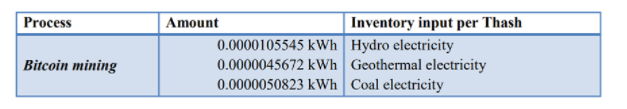
\includegraphics[width=.75\textwidth]{quellen/btc_mining_numbers.png}
    \caption[Energiemix für durchschnittliche ASIC]{Energiemix für durchschnittliche ASIC (\textit{Pollani Federica}, S.75)}
\end{figure}
\FloatBarrier
\noindent Diese Daten wurden dann in der Wirkungsabschätzung verwendet, um mithilfe der ReCiPe (H) Methode die Ecopoints für Bitcoins zu berechnen. Die berechneten Ecopoints für das gesamte Bitcoin-System in 2020 betrugen 1.358,41 MPt. Der gesamte Energiebedarf betrug 76,03 TWh \citebib{pollani}{S.76}{vgl. }.\\
Damit hat das Bitcoin-System deutlich größere Auswirkungen auf die Umwelt, als das gesamte Euro-Bargeld-System (59,98 MPt). Dennoch muss dieser Vergleich mit Vorsicht genossen werden. Die Studie hat lediglich ein Bargeldsystem mit nur einem Kryptowährungssystem verglichen. Auch ist zu beachten, dass der Euro hauptsächlich in Europa und der Bitcoin global verwendet und hergestellt wird. Nichtsdestotrotz lässt sich sagen, dass sich ein Wechsel von einem Bargeldsystem auf ein Kryptowährungssystem mit den aktuell verwendeten Berechnungsverfahren negativ auf die Umwelt auswirken würde.